\section{Synthetic Training-Data Augmentation}
\label{sec:augmentation}

\subsection{Research question and comparison}

Section~\ref{sec:mlp} asked whether a nonlinear MLP head improved prediction
when models were trained on real patients only. This section asks a different
question: whether adding generated records to each real training partition
changes the performance of the same model families, including the MLP. It is
therefore an augmentation experiment, not a second test of MLP architecture.
Performance is always measured in held-out real patients who were not used for
model training or synthetic-data generation. Four augmentation sizes were examined: 1,000,
5,000, 10,000 and 15,000 synthetic records.  Throughout this section, these
conditions are abbreviated as \texttt{+1K}, \texttt{+5K}, \texttt{+10K} and
\texttt{+15K}, where K denotes one thousand records.  Each augmented model was
compared with the same model trained on real data alone (\texttt{+0}).

\noindent\textbf{Data used in this section.} The starting data are the same
2,672-patient diagnostic and 462-patient prognostic SEER cohorts used in
Sections~\ref{sec:benchmark} and \ref{sec:mlp}. Within every evaluation fold or
split, a new synthetic pool is generated only from that fold's real training
patients. Models are trained on either the real training partition alone or the
combination of that real partition and a synthetic prefix. Evaluation uses only
the corresponding held-out real SEER patients. The full-cohort synthetic
datasets from Section~\ref{sec:transformations}, the precomputed embeddings and
the Erlangen cohort are not used here.

The analysis included the six diagnostic models and five prognostic models
evaluated in Sections~\ref{sec:benchmark} and \ref{sec:mlp}.  For diagnosis,
these were logistic regression, XGBoost, TabPFN-3, TabICLv2, TabDPT and the
clinical multilayer perceptron (MLP).  For prognosis, they were Cox elastic net,
random survival forest, TabPFN landmark, SurvivalPFN and the clinical MLP.  The
comparison therefore measures the effect of augmentation within each model; it
is not a new comparison of unrelated algorithms.

The main diagnostic outcomes were the area under the receiver operating
characteristic curve (ROC AUC), average precision (AP) and Brier score.  The
main prognostic outcomes were Uno's concordance index (Uno C), the 12-month
time-dependent AUC and the integrated Brier score (IBS) from 12 to 36 months.  Higher values
are favourable for discrimination measures, whereas lower Brier scores and IBS
values are favourable.  Calibration and decision-curve net benefit were
secondary outcomes.

The analysis comprised 875 primary model fits: 750 diagnostic fits from five
repeats of five-fold cross-validation and 125 prognostic fits from five held-out
splits.  Of these, 175 used real data alone and 700 used an augmented training
condition.  A further 300 MLP fits assessed sensitivity to three initialization
seeds.  All planned fits completed.  TabPFN representations that
had previously been generated from the full cohort were not included because
they did not preserve the training--test separation required for this
experiment.

\subsection{Training-partition-specific generation}
\label{sec:augmentation:construction}

Synthetic data were generated separately within every evaluation partition.
For diagnosis, one generator was fitted to the real training patients in each
of the 25 cross-validation folds.  For prognosis, one generator was fitted to
the real training patients in each of the five held-out splits.  Each generator
learned the distribution of the clinical predictors together with the relevant
outcome and produced a pool of 15,000 synthetic records.  The held-out real
patients were used only for evaluation and never entered the generator or an
augmented training set.

The four augmentation sizes were nested.  The \texttt{+1K} condition used the
first 1,000 records from a partition's synthetic pool, \texttt{+5K} used the
first 5,000, and so forth.  Every condition retained all real training records.
Using prefixes of the same pool makes the comparison across augmentation sizes
more direct because it avoids generating an unrelated synthetic sample for
each size.  The model seed was also held constant across sizes for the primary
comparison.

\begin{table}[htbp]
\centering\scriptsize
\setlength{\tabcolsep}{2.5pt}
\caption{Composition of the real-only and augmented training conditions.  Real
row counts and percentages are means across the 25 diagnostic or five
prognostic evaluation partitions.  Grade-4 prevalence decreases because no
grade-4 record was generated.}
\label{tab:augmentation:composition}
\begin{tabularx}{\linewidth}{@{}l rrr rrr@{}}
\toprule
& \multicolumn{3}{c}{Diagnosis (25 partitions)} &
  \multicolumn{3}{c}{Prognosis (5 partitions)} \\
\cmidrule(lr){2-4}\cmidrule(l){5-7}
Condition & Real rows & Synthetic share & Grade 4 & Real rows & Synthetic share & Grade 4 \\
\midrule
\csname @@input\endcsname{tables/synthetic_augmentation/condition_composition_rows.tex}
\bottomrule
\end{tabularx}
\end{table}

The effect on training-set composition differed markedly between tasks
(Table~\ref{tab:augmentation:composition}).  Diagnostic partitions contained a
mean of 2,138 real training records, so synthetic records represented 31.9\% of
the \texttt{+1K} condition and 87.5\% of \texttt{+15K}.  Prognostic partitions
contained only 323 real training records; synthetic records therefore already
represented 75.6\% at \texttt{+1K} and 97.9\% at \texttt{+15K}.  In the larger
prognostic conditions, model training was consequently dominated by the
generated distribution.

Preprocessing was learned separately within each training condition, using its
combined real and synthetic records and no held-out patients.  Synthetic data
could therefore affect which infrequent categorical levels were retained, the
number of encoded variables and the scaling parameters.  At \texttt{+1K}, a
category was retained only because of its synthetic frequency in 120 of 150
diagnostic and 15 of 25 prognostic preprocessing fits.  From \texttt{+5K}
onward, this occurred in all 150 diagnostic and all 25 prognostic fits.

For the MLP, training duration was chosen from the real training data only.  An
inner real-data split selected the number of epochs, after which the model was
reinitialized and trained for that fixed number of epochs on each complete
training condition.  The same epoch count was used across augmentation sizes
within a partition and seed.  This prevented synthetic validation records from
determining training duration, although larger conditions still required more
mini-batch updates per epoch.

\subsection{Synthetic-data quality and distributional similarity}
\label{sec:augmentation:fidelity}

All 30 partition-specific pools contained the expected 15,000 records and no
synthetic record exactly matched a real training record.  One duplicate pair
occurred within one diagnostic pool.  Two extremely large generated values
would not have been representable in the numerical format used for modelling;
each was therefore replaced by the corresponding minimum or maximum observed
in that partition's real training data.  These two replacements affected two
different pools.

Two variables were generated both in their original form and as a derived
clinical category.  At \texttt{+15K}, the tumour-size category did not agree
with the generated continuous tumour size in 1.47\% of diagnostic and 2.62\%
of prognostic synthetic records.  The binary indicator for positive nodal
stage disagreed with the generated N stage in approximately 0.001\% of records
for each task.  No such inconsistencies were present in the real training
records, and the synthetic inconsistencies were retained rather than corrected
before model fitting.

\begin{table}[htbp]
\centering\footnotesize
\caption{Quality checks for the 30 partition-specific synthetic pools.}
\label{tab:augmentation:integrity}
\begin{tabularx}{\linewidth}{@{}>{\RaggedRight\arraybackslash}p{4.2cm}>{\RaggedRight\arraybackslash}p{2.4cm}Y@{}}
\toprule
Check & Result & Scope or interpretation \\
\midrule
\csname @@input\endcsname{tables/synthetic_augmentation/integrity_rows.tex}
\bottomrule
\end{tabularx}
\end{table}

Table~\ref{tab:augmentation:fidelity} compares each synthetic prefix with the
real training records from which it was generated.  Jensen--Shannon divergence
(JSD) measures differences in categorical proportions and equals zero when the
two distributions match exactly.  The standardized Wasserstein distance
measures differences in continuous variables relative to the standard
deviation in the real training data.  The reported correlation difference is
the mean absolute difference between the Pearson correlation matrices of age,
tumour size and grade.

\begin{table}[htbp]
\centering\scriptsize
\setlength{\tabcolsep}{3pt}
\caption{Differences between synthetic and real training distributions.  JSD
uses base 2, and Wasserstein distances are divided by the standard deviation in
the corresponding real training partition.  Outcome and survival-time shifts
are calculated as synthetic minus real.}
\label{tab:augmentation:fidelity}
\begin{tabularx}{\linewidth}{@{}>{\RaggedRight\arraybackslash}p{0.45\linewidth}*{4}{>{\centering\arraybackslash}X}@{}}
\toprule
& \multicolumn{2}{c}{Diagnosis} & \multicolumn{2}{c}{Prognosis} \\
\cmidrule(lr){2-3}\cmidrule(l){4-5}
Measure & +1K & +15K & +1K & +15K \\
\midrule
\csname @@input\endcsname{tables/synthetic_augmentation/fidelity_rows.tex}
\bottomrule
\end{tabularx}
\end{table}

Overall differences changed little as more synthetic records were included.
Mean categorical JSD was 0.004 for diagnosis and 0.006 for prognosis at both
displayed sizes.  Grade was the main exception, with JSD values of
0.063--0.064 for diagnosis and 0.094--0.095 for prognosis because grade 4 was
absent from every synthetic pool.  Continuous-variable and correlation
differences were slightly smaller at \texttt{+15K}, which is consistent with
less random variation in the larger synthetic prefixes but does not correct the
missing grade-4 support.  At \texttt{+15K}, the synthetic liver-metastasis rate
was 2.04 percentage points below the corresponding real diagnostic training
rate.  In prognosis, the synthetic death-event rate was 1.01 percentage points
higher and median observed survival was 7.0 months longer than in the real
training data.

\begin{figure}[htbp]
\centering
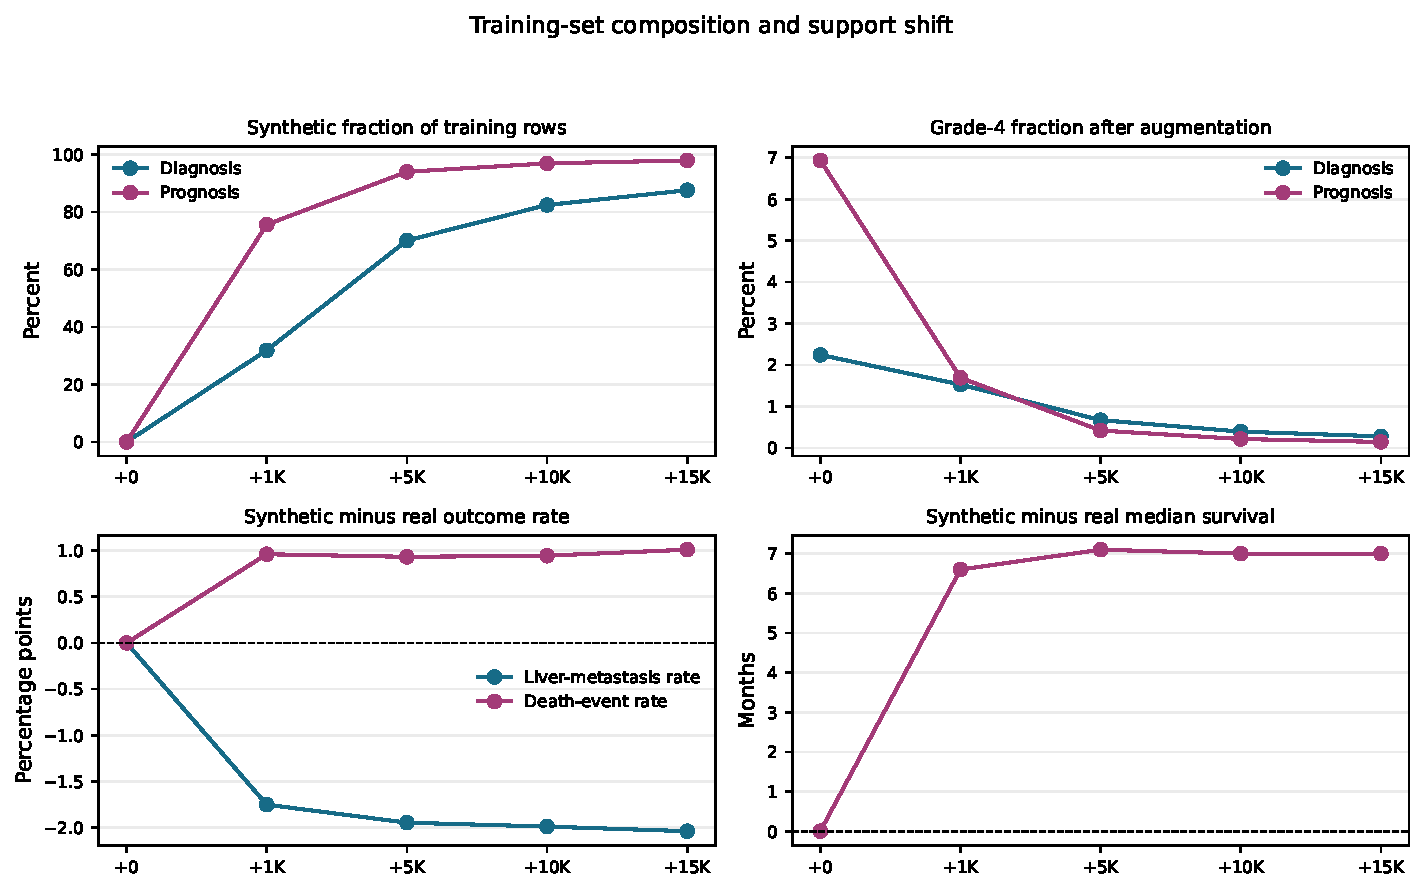
\includegraphics[width=0.98\linewidth]{synthetic_augmentation/augmentation_composition_shift.pdf}
\caption{Changes in training-set composition across augmentation sizes.  The
synthetic share rises faster for prognosis because its real training partitions
are smaller.  Grade-4 prevalence approaches zero, while outcome prevalence and
median observed survival remain shifted relative to the real training data.}
\label{fig:augmentation:composition}
\end{figure}

\subsection{Diagnostic performance}
\label{sec:augmentation:diagnostic}

Diagnostic effects depended on the model rather than showing a uniform benefit
(Table~\ref{tab:augmentation:diagnostic} and Figure
\ref{fig:augmentation:diagnostic}).  XGBoost showed the clearest improvement.
From \texttt{+0} to \texttt{+15K}, its ROC AUC increased from 0.883 to 0.895,
a paired change of 0.0126 with a 95\% interval of 0.0074 to 0.0180.  Average
precision increased by 0.0249 (0.0077 to 0.0433), and Brier score decreased
from 0.0961 to 0.0901.  Expressed so that positive values favour augmentation,
the Brier improvement was 0.0060 (0.0035 to 0.0086).  The AUC and Brier gains
were already evident at \texttt{+1K} and increased with augmentation size.
Despite this improvement, XGBoost's \texttt{+15K} AUC remained below the
approximately 0.900--0.901 values of the three tabular foundation models.

\begin{table}[htbp]
\centering\scriptsize
\setlength{\tabcolsep}{2.3pt}
\caption{Diagnostic results for real-only and maximum augmentation.  Paired
changes compare \texttt{+15K} with the same model at \texttt{+0}; positive
values favour augmentation.  Intervals are pointwise 95\% patient-bootstrap
intervals conditional on the fitted models.}
\label{tab:augmentation:diagnostic}
\begin{tabularx}{\linewidth}{@{}>{\RaggedRight\arraybackslash}p{2.1cm}rrYYY@{}}
\toprule
Model & AUC +0 & AUC +15K & $\Delta$ AUC [95\% interval] &
$\Delta$ AP [95\% interval] & Brier improvement [95\% interval] \\
\midrule
\csname @@input\endcsname{tables/synthetic_augmentation/diagnostic_endpoint_rows.tex}
\bottomrule
\end{tabularx}
\end{table}

Logistic regression and the clinical MLP showed little evidence of change.  At
\texttt{+15K}, their AUC changes were 0.0009 ($-0.0013$ to 0.0033) and 0.0013
($-0.0023$ to 0.0051), respectively, and the average-precision and Brier-score
intervals also included zero.  TabPFN-3 deteriorated slightly: its AUC change
was $-0.0027$ ($-0.0051$ to $-0.0001$), and its Brier improvement was
$-0.0016$ ($-0.0027$ to $-0.0007$).  Its AUC, average precision and Brier score
were already worse at \texttt{+1K}.  TabICLv2 also had a worse Brier score at
every augmented size, reaching a change of $-0.0014$ ($-0.0025$ to
$-0.0003$) at \texttt{+15K}, while its AUC change remained inconclusive.
TabDPT showed a small Brier deterioration at \texttt{+5K}, but its
\texttt{+15K} intervals included zero.

\begin{figure}[htbp]
\centering
\makebox[\linewidth][c]{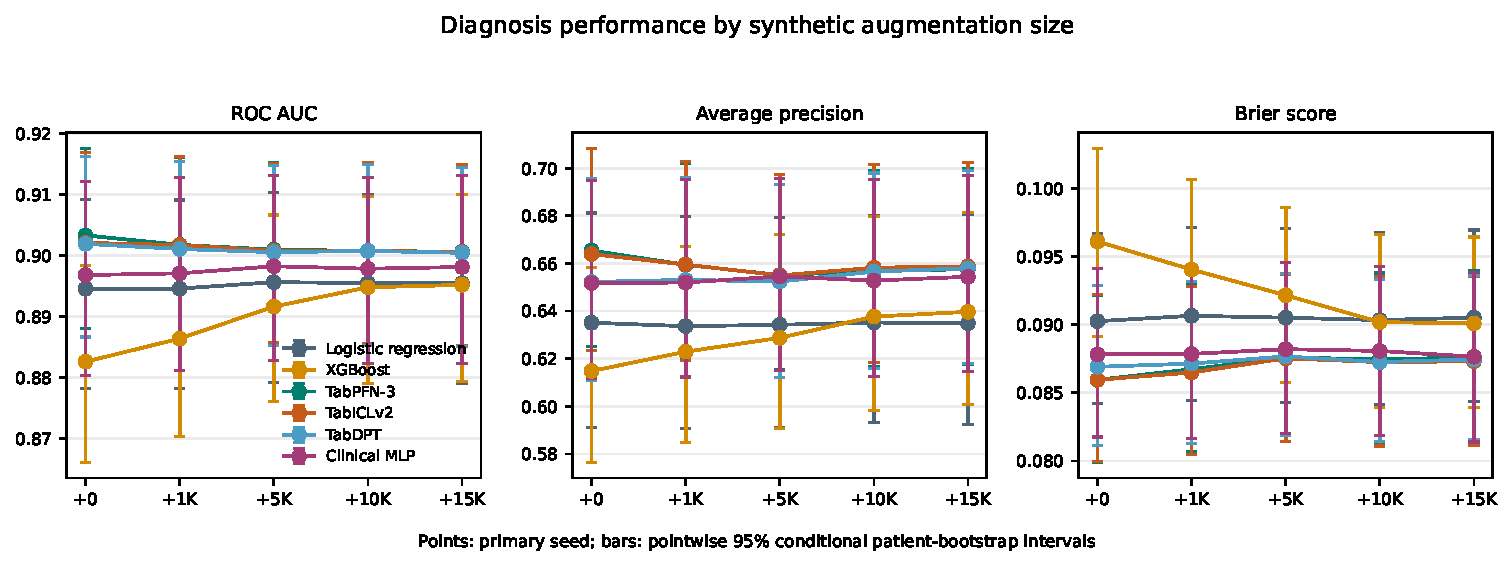
\includegraphics[width=1.05\linewidth]{synthetic_augmentation/augmentation_diagnostic_performance.pdf}}
\caption{Diagnostic performance across nested augmentation sizes.  Points are
primary-seed estimates, and bars are pointwise 95\% patient-bootstrap intervals
conditional on the fitted models.  The \texttt{+0} condition is the matched
real-only result for each model.}
\label{fig:augmentation:diagnostic}
\end{figure}

These results show that synthetic records were not equivalent to additional
independent patients.  They helped the initially weaker XGBoost classifier,
had little effect on logistic regression and the clinical MLP, and slightly
worsened the strongest diagnostic foundation models.  Because the generator
learned from the same finite real training sample, larger prefixes primarily
repeated and smoothed patterns inferred from that sample; they could not add
new clinical information beyond it.

\subsection{Prognostic performance}
\label{sec:augmentation:prognostic}

No model showed a clear improvement across the main prognostic outcomes
(Table~\ref{tab:augmentation:prognostic} and Figure
\ref{fig:augmentation:prognostic}).  Cox elastic net deteriorated from
\texttt{+5K} onward.  At \texttt{+15K}, Uno's concordance index fell from
0.711 to 0.686, a paired change of $-0.0250$ (95\% interval $-0.0477$ to
$-0.0010$).  IBS increased from 0.160 to 0.182; when oriented so that positive
values favour augmentation, the paired change was $-0.0214$ ($-0.0335$ to
$-0.0098$).  Its 12-month AUC also decreased by 0.0554 ($-0.0991$ to
$-0.0171$).

\begin{table}[htbp]
\centering\scriptsize
\setlength{\tabcolsep}{2.1pt}
\caption{Prognostic results for real-only and maximum augmentation.  Paired
changes compare \texttt{+15K} with the same model at \texttt{+0}; positive
values favour augmentation.  IBS improvement is real-only minus augmented IBS.}
\label{tab:augmentation:prognostic}
\begin{tabularx}{\linewidth}{@{}>{\RaggedRight\arraybackslash}p{2.35cm}rrYrrY@{}}
\toprule
Model & Uno C +0 & Uno C +15K & $\Delta$ Uno C [95\% interval] &
IBS +0 & IBS +15K & IBS improvement [95\% interval] \\
\midrule
\csname @@input\endcsname{tables/synthetic_augmentation/prognostic_endpoint_rows.tex}
\bottomrule
\end{tabularx}
\end{table}

For the clinical MLP, the concordance intervals included zero, but IBS was
worse at every augmented size.  The IBS-oriented improvement was $-0.0095$
($-0.0153$ to $-0.0038$) at \texttt{+1K} and $-0.0136$ ($-0.0216$ to
$-0.0058$) at \texttt{+15K}.  Random survival forest had a small IBS
deterioration at \texttt{+1K}; its larger-size concordance and IBS intervals
included zero.  TabPFN landmark was the most stable model.  At \texttt{+15K},
its concordance change was $-0.0006$ ($-0.0080$ to 0.0080), IBS improvement
was 0.0020 ($-0.0020$ to 0.0062), and 12-month AUC change was 0.0113
($-0.0011$ to 0.0239).  SurvivalPFN likewise showed no supported change at the
maximum augmentation size.

\begin{figure}[htbp]
\centering
\makebox[\linewidth][c]{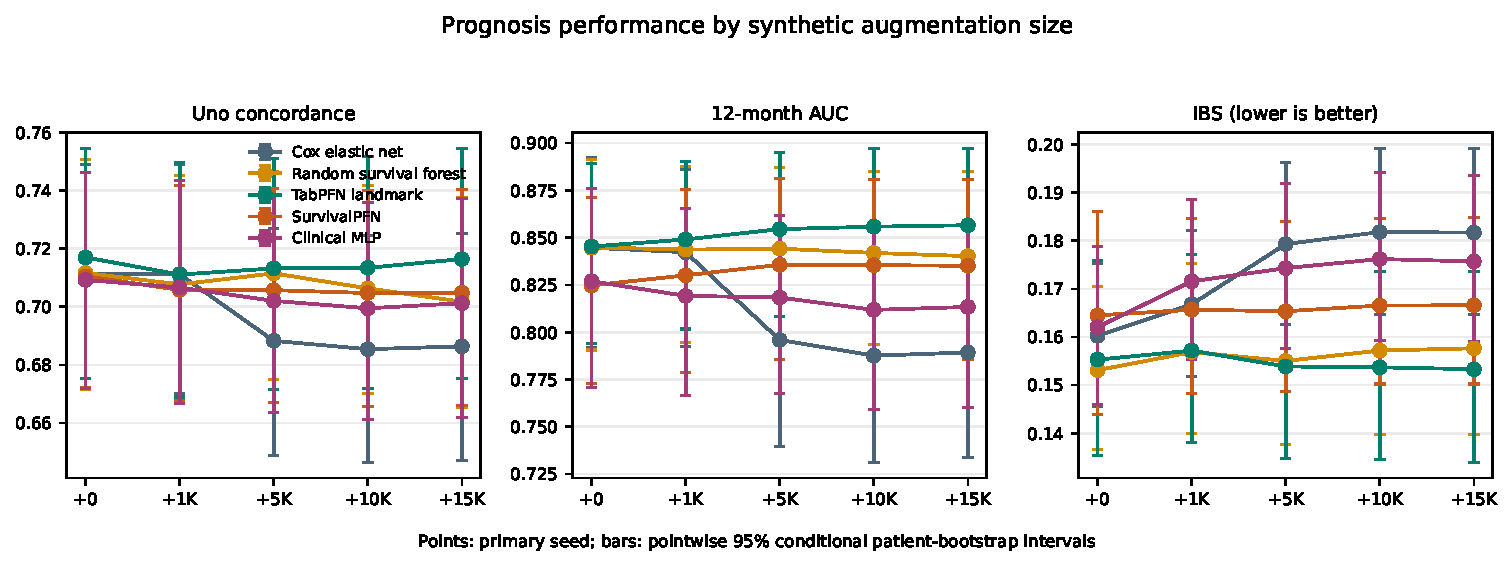
\includegraphics[width=1.05\linewidth]{synthetic_augmentation/augmentation_prognostic_performance.pdf}}
\caption{Prognostic performance across nested augmentation sizes.  Points are
primary-seed estimates, and bars are pointwise 95\% patient-bootstrap intervals
conditional on the fitted models.  Lower IBS is favourable.}
\label{fig:augmentation:prognostic}
\end{figure}

The more pronounced deterioration in prognosis occurred while synthetic
records made up a much larger share of training than in diagnosis.  This
association does not identify a single cause.  Outcome shifts, missing grade-4
support, inconsistencies between linked variables, preprocessing changes and
repeated emphasis of patterns learned from the small real training sample all
changed together.  The results therefore describe the complete augmentation
procedure rather than the isolated effect of any one difference.

\subsection{Paired effects, calibration and decision-curve results}
\label{sec:augmentation:calibration}

Paired intervals were calculated with 2,000 bootstrap resamples of the real
evaluation patients.  The same resample was used for an augmented fit and its
real-only reference, preserving the patient-level pairing.  These intervals
quantify evaluation-sample variation while treating the trained models and
synthetic pools as fixed.  Figure~\ref{fig:augmentation:paired} summarizes the
main paired changes on a common scale where positive values favour
augmentation.  It shows the increasing diagnostic benefit for XGBoost, the
worsening prognostic error for Cox elastic net and the MLP, and changes close to
zero for most other comparisons.

\begin{figure}[htbp]
\centering
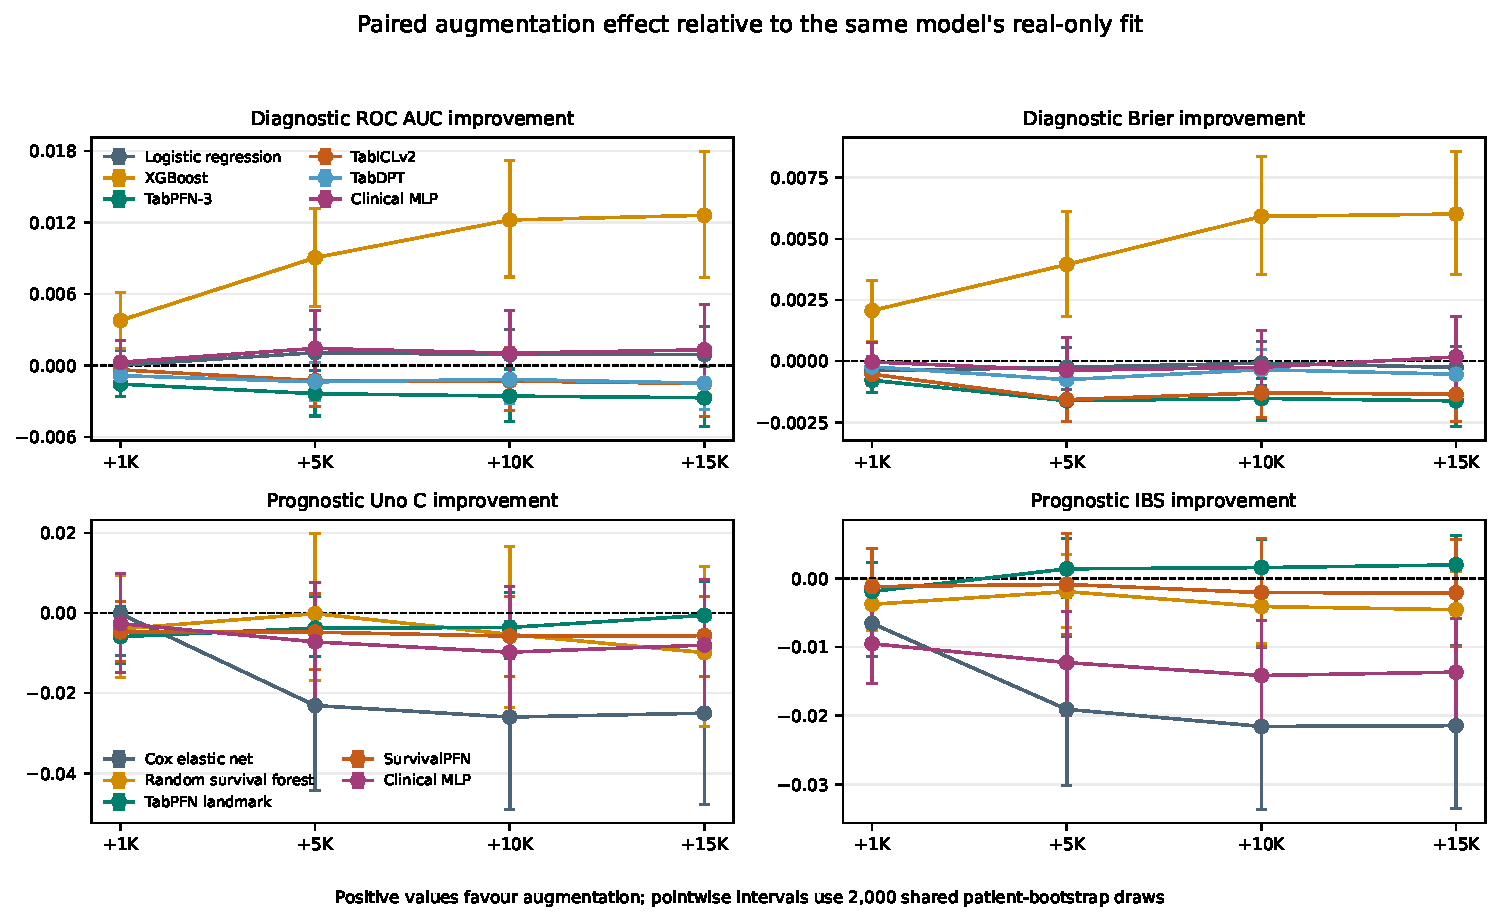
\includegraphics[width=\linewidth]{synthetic_augmentation/augmentation_paired_improvements.pdf}
\caption{Paired effect of each augmentation size relative to the same model
trained on real data alone.  Positive values favour augmentation.  Intervals
are pointwise 95\% patient-bootstrap intervals conditional on the fitted
models; they are not adjusted for the number of models, outcomes or sizes.}
\label{fig:augmentation:paired}
\end{figure}

Diagnostic calibration also varied by model
(Table~\ref{tab:augmentation:calibration}).  A calibration slope of one is
ideal.  XGBoost's slope moved from 0.731 to 0.878, reducing its absolute
distance from one by 0.1479 (0.1184 to 0.1801).  In contrast, TabPFN-3 moved
from 0.899 to 0.851 and TabICLv2 from 0.910 to 0.868; for both models, the
change away from one had an interval excluding zero.  Changes for logistic
regression, TabDPT and the MLP were inconclusive at \texttt{+15K}.

For prognosis, calibration was summarized as the mean absolute difference
between predicted survival and the Kaplan--Meier (KM) estimate across three
risk groups and the 12-, 24- and 36-month horizons.  The mean gap increased
from 0.069 to 0.086 for Cox elastic net and from 0.065 to 0.086 for the MLP,
remained 0.044 for random survival forest, decreased from 0.054 to 0.049 for
TabPFN landmark, and changed from 0.052 to 0.054 for SurvivalPFN.  These are
descriptive point estimates.  The planned bootstrap intervals were not
reported because fewer than 1,900 of the 2,000 resamples retained at least five
patients at risk in every required risk-group and time-horizon cell.

\begin{table}[htbp]
\centering\scriptsize
\setlength{\tabcolsep}{2.6pt}
\caption{Calibration for real-only and maximum augmentation.  Diagnostic
improvement is the reduction in the absolute distance of the slope from one.
Prognostic KM gaps are descriptive because the required number of valid
bootstrap resamples was not reached.}
\label{tab:augmentation:calibration}
\begin{tabularx}{\linewidth}{@{}>{\RaggedRight\arraybackslash}p{1.45cm}>{\RaggedRight\arraybackslash}p{2.15cm}>{\RaggedRight\arraybackslash}p{2.7cm}rrY@{}}
\toprule
Task & Model & Metric & +0 & +15K & Paired change [95\% interval] \\
\midrule
\csname @@input\endcsname{tables/synthetic_augmentation/calibration_rows.tex}
\bottomrule
\end{tabularx}
\end{table}

\begin{figure}[htbp]
\centering
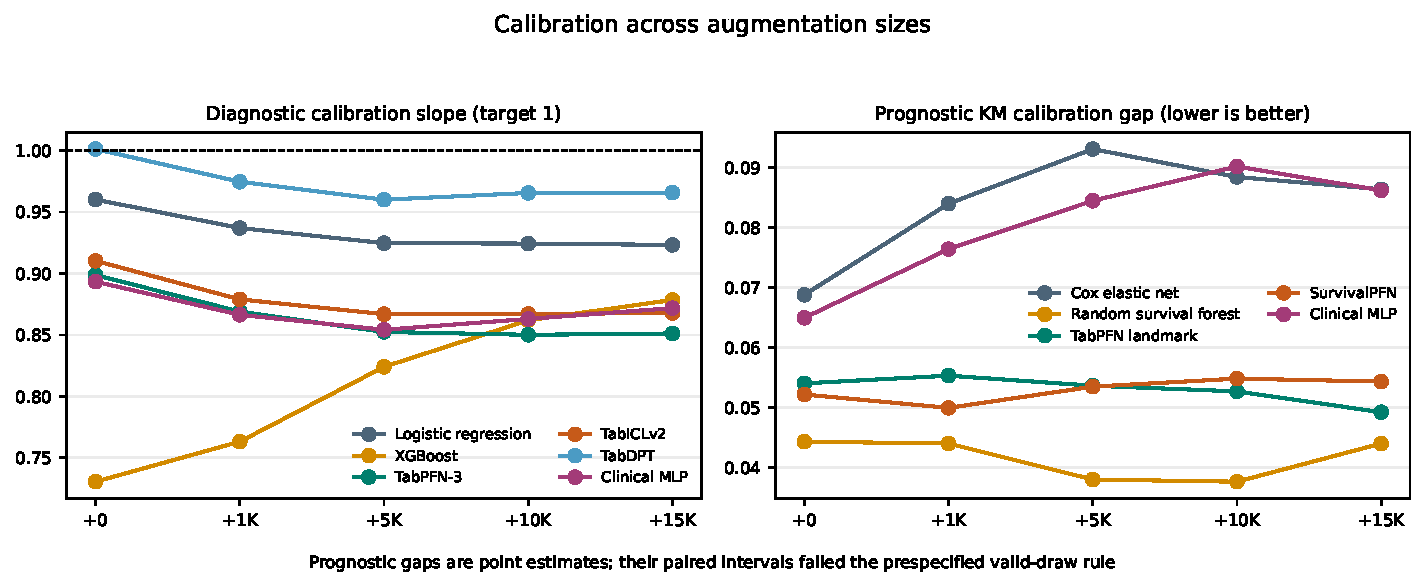
\includegraphics[width=0.98\linewidth]{synthetic_augmentation/augmentation_calibration.pdf}
\caption{Diagnostic calibration slope and prognostic mean absolute KM
calibration gap across augmentation sizes.  The target is one for diagnostic
slope and zero for prognostic gap.  Prognostic curves are descriptive because
the planned bootstrap intervals did not meet the valid-resample requirement.}
\label{fig:augmentation:calibration}
\end{figure}

Diagnostic decision curves were summarized at risk thresholds of 0.10, 0.20
and 0.30 (Table~\ref{tab:augmentation:dca}).  Net benefit balances true-positive
detections against false-positive classifications at a chosen threshold.  At
\texttt{+15K}, XGBoost gained approximately 0.006--0.007 net-benefit units at
the three thresholds, whereas every other model changed by no more than about
0.0022 in either direction.  No bootstrap interval was planned for these
summaries, so they provide descriptive evidence only and do not establish
clinical utility in another population.

\begin{table}[htbp]
\centering\footnotesize
\caption{Descriptive change in diagnostic net benefit from \texttt{+0} to
\texttt{+15K}.  Positive values favour augmentation.}
\label{tab:augmentation:dca}
\begin{tabular}{@{}lrrr@{}}
\toprule
Model & Threshold 0.10 & Threshold 0.20 & Threshold 0.30 \\
\midrule
\csname @@input\endcsname{tables/synthetic_augmentation/decision_curve_rows.tex}
\bottomrule
\end{tabular}
\end{table}

\subsection{Grade-4 support, MLP seed sensitivity and computation}
\label{sec:augmentation:robustness}

Augmentation did not resolve the limited grade-4 support.  Grade 4 was absent
from every synthetic pool, so its mean prevalence in the combined training
data fell from 2.25\% to 0.28\% for diagnosis and from 6.93\% to 0.15\% for
prognosis between \texttt{+0} and \texttt{+15K}.  Fold-level diagnostic grade-4
metrics were estimable in only 44 of 1,100 model-by-fold conditions.  When
predictions were combined across the five folds in each repeat, all 220
model-by-repeat conditions could be summarized.  At this repeat level,
XGBoost's grade-4 AUC increased descriptively from 0.533 to 0.591 and Brier
score decreased from 0.319 to 0.270 at \texttt{+15K}.  However, each repeat
contained only 60 unique grade-4 patients, no paired interval was available,
and the models received no synthetic grade-4 examples.  These estimates are
therefore too limited to support a grade-4 benefit.  Prognostic grade-4 metrics
could not be estimated in any held-out split.

Three MLP initialization seeds were examined as a focused sensitivity analysis
(Table~\ref{tab:augmentation:mlp-seeds}).  Diagnostic AUC changes were small
and positive at \texttt{+5K} and \texttt{+15K} for all three seeds, while
Brier-score changes varied in direction.  Prognostic IBS increased, indicating
worse probability accuracy, for every seed at both sizes.  Concordance changes
were mostly negative, with one small positive change at \texttt{+15K}.  The
consistent direction of the prognostic IBS result supports the primary-seed
finding, although three seeds cannot represent the full range of optimization
variability.

\begin{table}[htbp]
\centering\footnotesize
\caption{MLP metric changes from the real-only fit for seeds 20230529,
20230530 and 20230531.  Values are descriptive seed-specific changes rather
than confidence intervals.  Positive values favour AUC and Uno concordance but
are unfavourable for Brier score and IBS.}
\label{tab:augmentation:mlp-seeds}
\begin{tabularx}{\linewidth}{@{}>{\RaggedRight\arraybackslash}p{3.3cm}YY@{}}
\toprule
Metric & +5K minus +0 & +15K minus +0 \\
\midrule
\csname @@input\endcsname{tables/synthetic_augmentation/mlp_seed_rows.tex}
\bottomrule
\end{tabularx}
\end{table}

Larger training conditions increased fit-and-prediction time for most models
(Table~\ref{tab:augmentation:runtime}).  Among the diagnostic models, the three
foundation models and the MLP took 5.4--6.5 times longer at \texttt{+15K}; for
example, the median TabPFN-3 time increased from 2.82 to 16.25 seconds per
cross-validation fold.  In prognosis, TabPFN landmark increased from 5.81 to
35.56 seconds per split, while SurvivalPFN and the MLP increased by a factor of
1.3.  All models assigned to graphics-processing-unit execution completed the
largest condition without falling back to central-processing-unit execution.
The largest recorded graphics-memory allocation was 2.58~GB for TabICLv2.
These measurements describe the present implementation and hardware; they do
not provide a controlled speed comparison between algorithms.

\begin{table}[htbp]
\centering\scriptsize
\caption{Median fit-and-prediction time per evaluation partition.  Times
exclude synthetic-data generation, bootstrap calculations and report
preparation.}
\label{tab:augmentation:runtime}
\begin{tabularx}{\linewidth}{@{}>{\RaggedRight\arraybackslash}p{1.5cm}>{\RaggedRight\arraybackslash}p{4.4cm}*{3}{>{\RaggedLeft\arraybackslash}X}@{}}
\toprule
Task & Model & +0 (s) & +15K (s) & Ratio \\
\midrule
\csname @@input\endcsname{tables/synthetic_augmentation/runtime_rows.tex}
\bottomrule
\end{tabularx}
\end{table}

\subsection{Interpretation and limitations}
\label{sec:augmentation:limits}

The main finding is that synthetic augmentation had selective rather than
general value.  It improved XGBoost's diagnostic discrimination, Brier score,
calibration slope and descriptive net benefit.  It did not clearly improve
diagnostic logistic regression or the clinical MLP, and it slightly worsened
some results for TabPFN-3 and TabICLv2.  No prognostic model showed a clear
overall benefit.  In particular, Cox elastic net and the clinical MLP had worse
probability accuracy as synthetic records came to dominate the training data.
TabPFN landmark was comparatively stable, but stability should not be
interpreted as improvement.

The uncertainty intervals have several limits.  They reflect variation among
the held-out real patients while treating the fitted models, selected MLP epoch
counts and generated pools as fixed.  They therefore do not include uncertainty
from retraining the models or generator.  The intervals are pointwise and were
not adjusted for the number of models, outcomes and augmentation sizes.  In
addition, increasing the synthetic prefix simultaneously changed sample size,
outcome distribution, grade support, categorical encoding, scaling and
computational effort.  The observed curves cannot identify which of these
changes caused a performance difference.

The generated data also omitted grade 4, contained small inconsistencies
between linked variables and accounted for 97.9\% of the rows in the largest
prognostic training conditions.  Finally, every result was
evaluated within the same Surveillance, Epidemiology, and End Results (SEER)
registry cohort.  The analysis therefore addresses internal predictive
performance and does not establish transportability or clinical utility in an
independent population.

Taken together, the results show that synthetic augmentation must be evaluated
for the specific model and clinical task in which it will be used.  Close
agreement in overall feature distributions did not guarantee better
discrimination, calibration, probability accuracy or subgroup support.  The
next section combines these findings with the real-only, transformed-data,
foundation-model and nonlinear-head experiments.

\FloatBarrier
